\documentclass{beamer}
\beamertemplatenavigationsymbolsempty
%\setbeamertemplate{navigation symbols}{}
\usecolortheme{beaver}
\setbeamertemplate{blocks}[rounded=true, shadow=true]
\setbeamertemplate{footline}[page number]

\usepackage{cmap}
\usepackage[T2A]{fontenc}
\usepackage[utf8]{inputenc}
\usepackage[english,russian]{babel}
\usepackage{amsmath,mathrsfs,amsfonts,amssymb}
\usepackage{graphicx, epsfig,subfig}
\usepackage[noend]{algorithmic}
\usepackage{multicol}
\usepackage{array}
\usepackage{hhline}
\graphicspath{ {fig/} }

\newcommand{\T}{^{\text{\tiny\sffamily\upshape\mdseries T}}}
\newcommand\argmin{\mathop{\arg\min}}
\newcommand{\A}{\mathcal{A}}
\newcommand{\hchi}{\hat{\boldsymbol{\chi}}}
\newcommand{\hphi}{\hat{\boldsymbol{\varphi}}}
\newcommand{\B}{\mathcal{B}}
\newcommand{\hx}{\hat{x}}
\newcommand{\hy}{\hat{y}}
\newcommand{\SM}{\mathbf{S}}

\def\algorithmicrequire{\textbf{\textcolor[rgb]{0.00,0.00,1.00}{Вход:}}}
\def\algorithmicensure{\textbf{\textcolor[rgb]{0.00,0.00,1.00}{Выход:}}}

\title{Согласование прогнозов в задачах прогнозирования иерархических временных рядов (пример)}
\author{Мария Стенина}
\institute[МФТИ]{Московский физико-технический институт \\ Физтех-школа прикладной математики и информатики\\  Кафедра интеллектуальных систем 
\vspace{0.3cm} \\
Научный руководитель д.ф.-м.н. В.\,В.\,Cтрижов}
\date{61-я Всероссийская научная конференция МФТИ\\
	Москва, 2020}

\begin{document}
% Creates title page of slide show using above information
\begin{frame}
  \titlepage
\end{frame}
%----------------------------------------------------------------------------------------------------
%\section{Постановка задачи}
\begin{frame}{Цель работы}
    \footnotesize
    \begin{block}{Задача}
        Построить прогнозы семейства временных рядов, связанных в
        иерархическую многоуровневую структуру и описывающих
        объемы погрузки ряда грузов в заданных узлах
        РЖД с разным уровнем детализации.
    \end{block}
    \vfill
%    Требуется построить прогнозы
%    \begin{enumerate}
%        \item погрузки каждого типа груза на каждом
%        железнодорожном узле
%        по отдельности;
%        \item суммарной погрузки всех грузов на заданном ЖД-узле
%        (для каждого узла);
%        \item суммарной погрузки груза на всех ЖД-узлах (для каждого типа
%        груза).
%    \end{enumerate}

    \begin{block}{Требования к модели}
        \begin{itemize}
            \item прогнозы должны быть точны --- обеспечивать минимально возможное значение заданной
            функции потерь;
            \item прогнозы должны удовлетворять физическим
            ограничениям --- лежать в заданном интервале для каждого временного ряда;
            \item прогнозы должны удовлетворять условию
            согласованности (структуре иерархии).
        \end{itemize}
    \end{block}

    \begin{block}{Проблема согласования прогнозов}
        Прогнозы, полученные для каждого временного ряда
        независимо, могут не удовлетворять структуре иерархии, т. е.
        не быть \emph{согласованными}.
    \end{block}
\end{frame}
%----------------------------------------------------------------------------------------------------
\begin{frame}{Условие согласованности прогнозов}
	\begin{columns}[c]
		\column{0.6\textwidth}
		\includegraphics[width=1.1\textwidth, viewport= 4.5cm 10cm 20.2cm 25.3cm, clip]{Hierarchy3Levels.eps}
		\column{0.4\textwidth}
        {\small
        \textcolor[rgb]{0.00,0.00,1.00}{$x_t(:, :) = \sum\limits_{i = 1}^n x_t(i, :);$} \\ %\vspace{0.2cm} 

        \textcolor[rgb]{1.00,0.00,1.00}{$x_t(:, :) = \sum\limits_{j = 1}^m x_t(:, j);$} \\%\vspace{0.2cm}

        \textcolor[rgb]{1.00,0.00,0.00}{$x_t(i, :) = \sum\limits_{j = 1}^m x_t(i, j),$} \\

        ~~~~~~~~~~~~~ {\tiny\textcolor[rgb]{1.00,0.00,0.00}{$i = 1, \ldots n;$}}  \\ %\vspace{0.1cm}

        \textcolor[rgb]{0.00,0.59,0.00}{$x_t(:, j) = \sum\limits_{i = 1}^n x_t(i, j),$} \\

        ~~~~~~~~~~~~~ {\tiny\textcolor[rgb]{0.00,0.59,0.00}{$j = 1, \ldots m;$}}  \\%\vspace{0.05cm}
        $t = 1, \ldots, T.$
		}
       % \vspace{0.3cm}
       \includegraphics[width=\textwidth]{TimeSeriesExample.eps}
	\end{columns}
%   \begin{block}{Проблема согласования прогнозов}
%        Для прогнозов, полученных для каждого временного ряда
%        независимо, условие согласованности может не выполняться.
%        Необходимо скорректировать прогнозы так, чтобы это условие
%        выполнилось.
%    \end{block}
\end{frame}
%----------------------------------------------------------------------------------------------------
\begin{frame}{Существующие решения}
    \small
    \textbf{Алгоритмы согласования прогнозов}
    \begin{enumerate}
        \item Albert B. Schwarzkopf, Richard J. Tersine, John S.
        Morris \textit{Top-down versus
        bottom-up forecasting strategies.} The International Journal Of
        Production Research, 26(11):1833–-1843, 1988.
        \item Rob J. Hyndman, Roman A. Ahmed, George Athanasopoulos, Han Lin Shang. \textit{Optimal
        combination forecasts for hierarchical time series.} Computational
        Statistics and Data Analysis, 55(9):2579–2589, 2011.
    \end{enumerate}

    \textbf{Базовые публикации}
    \begin{enumerate}
        \item Tim Van Erven and Jairo Cugliari. Game-theoretically optimal reconciliation of contemporaneous
        hierarchical time series forecasts. 2013.
        \item М.\,М. Стенина, В.\,В. Стрижов. \textit{Согласование агрегированных и
        детализированных прогнозов при решении задач непараметрического прогнозирования.}
        Системы и средства информатики, 24(2):21–34, 2014.
    \end{enumerate}
\end{frame}
%----------------------------------------------------------------------------------------------------
%\subsection{Обозначения}
\begin{frame}{Обозначения: структура иерархии}

    \textbf{Срез иерархии, вектор независимых и вектор согласованных
    прогнозов:} \vspace{0.1cm}

    {\small
    $\boldsymbol{\chi}_t = \left(%
                        \begin{array}{c}
                        x_t(:, :) \\
                        \ldots \\
                        x_t(n, 1) \\
                        \ldots \\
                        x_t(n, m) \\
                        \end{array}%
                      \right),~
            \hchi = \left(%
                    \begin{array}{c}
                        \hat{x}(:, :) \\
                        \ldots \\
                        \hat{x}(n, 1) \\
                        \ldots \\
                        \hat{x}(n, m) \\
                    \end{array}%
                    \right),~
            \hphi = \left(%
                    \begin{array}{c}
                        \hat{y}(:, :) \\
                        \ldots \\
                        \hat{y}(n, 1) \\
                        \ldots \\
                        \hat{y}(n, m) \\
                    \end{array}%
                    \right).$}

    \vspace{0.3cm}
    Условие согласованности~~~~~~$\textcolor[rgb]{1.00,0.00,0.00}{\SM} \boldsymbol{\chi}_t =
        \boldsymbol{0}, ~ t = 1, \ldots, T,$

    \vspace{0.2cm}
    где \textcolor[rgb]{1.00,0.00,0.00}{$\SM$~--- матрица связей}, имеет размер $(2 + n + m) \times (1 + n + m +
    nm)$ и записывается в виде
    \scriptsize
    $$
        \textcolor[rgb]{1.00,0.00,0.00}{\SM} = \left(%
        \begin{array}{c|ccc|ccc|cccc|c|cccc}
            \textcolor[rgb]{0.00,0.00,1.00}{-1} &
            \textcolor[rgb]{0.00,0.00,1.00}{1} &
            \textcolor[rgb]{0.00,0.00,1.00}{\ldots} &
            \textcolor[rgb]{0.00,0.00,1.00}{1} &
            \textcolor[rgb]{0.00,0.00,1.00}{0} &
            \textcolor[rgb]{0.00,0.00,1.00}{\ldots} &
            \textcolor[rgb]{0.00,0.00,1.00}{0} &
            \textcolor[rgb]{0.00,0.00,1.00}{0} &
            \textcolor[rgb]{0.00,0.00,1.00}{0} &
            \textcolor[rgb]{0.00,0.00,1.00}{\ldots} &
            \textcolor[rgb]{0.00,0.00,1.00}{0} &
            \textcolor[rgb]{0.00,0.00,1.00}{\ldots} &
            \textcolor[rgb]{0.00,0.00,1.00}{0} &
            \textcolor[rgb]{0.00,0.00,1.00}{0} &
            \textcolor[rgb]{0.00,0.00,1.00}{\ldots} &
            \textcolor[rgb]{0.00,0.00,1.00}{0} \\

            \textcolor[rgb]{1.00,0.00,1.00}{-1} &
            \textcolor[rgb]{1.00,0.00,1.00}{0} &
            \textcolor[rgb]{1.00,0.00,1.00}{\ldots} &
            \textcolor[rgb]{1.00,0.00,1.00}{0} &
            \textcolor[rgb]{1.00,0.00,1.00}{1} &
            \textcolor[rgb]{1.00,0.00,1.00}{\ldots} &
            \textcolor[rgb]{1.00,0.00,1.00}{1} &
            \textcolor[rgb]{1.00,0.00,1.00}{0} &
            \textcolor[rgb]{1.00,0.00,1.00}{0} &
            \textcolor[rgb]{1.00,0.00,1.00}{\ldots} &
            \textcolor[rgb]{1.00,0.00,1.00}{0} &
            \textcolor[rgb]{1.00,0.00,1.00}{\ldots} &
            \textcolor[rgb]{1.00,0.00,1.00}{0} &
            \textcolor[rgb]{1.00,0.00,1.00}{0} &
            \textcolor[rgb]{1.00,0.00,1.00}{\ldots} &
            \textcolor[rgb]{1.00,0.00,1.00}{0} \\

            \hline

            \textcolor[rgb]{1.00,0.00,0.00}{0} &
            \textcolor[rgb]{1.00,0.00,0.00}{-1} &
            \textcolor[rgb]{1.00,0.00,0.00}{\ldots} &
            \textcolor[rgb]{1.00,0.00,0.00}{0} &
            \textcolor[rgb]{1.00,0.00,0.00}{0} &
            \textcolor[rgb]{1.00,0.00,0.00}{\ldots} &
            \textcolor[rgb]{1.00,0.00,0.00}{0} &
            \textcolor[rgb]{1.00,0.00,0.00}{1} &
            \textcolor[rgb]{1.00,0.00,0.00}{1} &
            \textcolor[rgb]{1.00,0.00,0.00}{\ldots} &
            \textcolor[rgb]{1.00,0.00,0.00}{1} &
            \textcolor[rgb]{1.00,0.00,0.00}{\ldots} &
            \textcolor[rgb]{1.00,0.00,0.00}{0} &
            \textcolor[rgb]{1.00,0.00,0.00}{0} &
            \textcolor[rgb]{1.00,0.00,0.00}{\ldots} &
            \textcolor[rgb]{1.00,0.00,0.00}{0} \\

            \textcolor[rgb]{1.00,0.00,0.00}{\ldots} &
            &
            \textcolor[rgb]{1.00,0.00,0.00}{\ldots} &
            &
            &
            \textcolor[rgb]{1.00,0.00,0.00}{\ldots} &
            &
            &
            &
            \textcolor[rgb]{1.00,0.00,0.00}{\ldots} &
            &
            &
            &
            &
            \textcolor[rgb]{1.00,0.00,0.00}{\ldots} &  \\

            \textcolor[rgb]{1.00,0.00,0.00}{0} &
            \textcolor[rgb]{1.00,0.00,0.00}{0} &
            \textcolor[rgb]{1.00,0.00,0.00}{\ldots} &
            \textcolor[rgb]{1.00,0.00,0.00}{-1} &
            \textcolor[rgb]{1.00,0.00,0.00}{0} &
            \textcolor[rgb]{1.00,0.00,0.00}{\ldots} &
            \textcolor[rgb]{1.00,0.00,0.00}{0} &
            \textcolor[rgb]{1.00,0.00,0.00}{0} &
            \textcolor[rgb]{1.00,0.00,0.00}{0} &
            \textcolor[rgb]{1.00,0.00,0.00}{\ldots} &
            \textcolor[rgb]{1.00,0.00,0.00}{0} &
            \textcolor[rgb]{1.00,0.00,0.00}{\ldots} &
            \textcolor[rgb]{1.00,0.00,0.00}{1} &
            \textcolor[rgb]{1.00,0.00,0.00}{1} &
            \textcolor[rgb]{1.00,0.00,0.00}{\ldots} &
            \textcolor[rgb]{1.00,0.00,0.00}{1} \\

            \hline

            \textcolor[rgb]{0.00,0.50,0.00}{0} &
            \textcolor[rgb]{0.00,0.50,0.00}{0} &
            \textcolor[rgb]{0.00,0.50,0.00}{\ldots} &
            \textcolor[rgb]{0.00,0.50,0.00}{0} &
            \textcolor[rgb]{0.00,0.50,0.00}{-1} &
            \textcolor[rgb]{0.00,0.50,0.00}{\ldots} &
            \textcolor[rgb]{0.00,0.50,0.00}{0} &
            \textcolor[rgb]{0.00,0.50,0.00}{1} &
            \textcolor[rgb]{0.00,0.50,0.00}{0} &
            \textcolor[rgb]{0.00,0.50,0.00}{\ldots} &
            \textcolor[rgb]{0.00,0.50,0.00}{0} &
            \textcolor[rgb]{0.00,0.50,0.00}{\ldots} &
            \textcolor[rgb]{0.00,0.50,0.00}{1} &
            \textcolor[rgb]{0.00,0.50,0.00}{0} &
            \textcolor[rgb]{0.00,0.50,0.00}{\ldots} &
            \textcolor[rgb]{0.00,0.50,0.00}{0} \\

            \textcolor[rgb]{0.00,0.50,0.00}{\ldots} &
            &
            \textcolor[rgb]{0.00,0.50,0.00}{\ldots} &
            &
            &
            \textcolor[rgb]{0.00,0.50,0.00}{\ldots} &
            &
            &
            &
            \textcolor[rgb]{0.00,0.50,0.00}{\ldots} &
            &
            &
            &
            &
            \textcolor[rgb]{0.00,0.50,0.00}{\ldots} &  \\

            \textcolor[rgb]{0.00,0.50,0.00}{0} &
            \textcolor[rgb]{0.00,0.50,0.00}{0} &
            \textcolor[rgb]{0.00,0.50,0.00}{\ldots} &
            \textcolor[rgb]{0.00,0.50,0.00}{0} &
            \textcolor[rgb]{0.00,0.50,0.00}{0} &
            \textcolor[rgb]{0.00,0.50,0.00}{\ldots} &
            \textcolor[rgb]{0.00,0.50,0.00}{-1} &
            \textcolor[rgb]{0.00,0.50,0.00}{0} &
            \textcolor[rgb]{0.00,0.50,0.00}{0} &
            \textcolor[rgb]{0.00,0.50,0.00}{\ldots} &
            \textcolor[rgb]{0.00,0.50,0.00}{1} &
            \textcolor[rgb]{0.00,0.50,0.00}{\ldots} &
            \textcolor[rgb]{0.00,0.50,0.00}{0} &
            \textcolor[rgb]{0.00,0.50,0.00}{0} &
            \textcolor[rgb]{0.00,0.50,0.00}{\ldots} &
            \textcolor[rgb]{0.00,0.50,0.00}{1} \\
        \end{array}%
        \right).
    $$

    %Рассмотрим плоскую двухуровневую иерархию. Такой вид имеет отдельный узел любой более сложной иерархии.
%    \vspace{0.1cm}
%
%    \begin{tabular}{cp{7.5cm}}
%        \raisebox{-1.5cm}{\includegraphics[width=0.33\textwidth, viewport= 4cm 21cm 13cm
%            26cm]{Hierarhy2Levels.ps}}
%            &
%            \textbf{Срез иерархии, вектор независимых и вектор
%            согласованных прогнозов}
%            \vspace{0.1cm}
%
%            \footnotesize
%            $\boldsymbol{\chi}_t = \left(%
%                        \begin{array}{c}
%                        x_t(:) \\
%                        x_t(1) \\
%                        \ldots \\
%                        x_t(n) \\
%                        \end{array}%
%                      \right),~
%            \hchi = \left(%
%                    \begin{array}{c}
%                        \hat{x}(:) \\
%                        \hat{x}(1) \\
%                        \ldots \\
%                        \hat{x}(n) \\
%                    \end{array}%
%                    \right),~
%            \hphi = \left(%
%                    \begin{array}{c}
%                        \hat{y}(:) \\
%                        \hat{y}(1) \\
%                        \ldots \\
%                        \hat{y}(n) \\
%                    \end{array}%
%                    \right).$ \\
%    \end{tabular}
%    \vspace{0.2cm}
%
%    Условие согласованности $~~~~~x_t(:) = \sum\limits_{i=1}^n x_t(i), ~t = 1, \ldots,
%    T$ \vspace{0.1cm}
%
%    можно записать в виде $~~~~~\SM \boldsymbol{\chi}_t = 0, ~ t = 1, \ldots,
%    T,$ ~~~~~где
%    $$
%        \textcolor[rgb]{1.00,0.00,0.00}{\SM = \left(%
%            \begin{array}{cccc}
%            -1 & 1 & \ldots & 1 \\
%            \end{array}%
%            \right) \text{ --- матрица связей.}}
%    $$


    %\vspace{0.2cm}
%    Множество векторов, удовлетворяющих условию согласованности
%    $$
%        \textcolor[rgb]{1.00,0.00,0.00}{\A = \{ \boldsymbol{\chi} \in \mathbb{R}^d \mid \SM \boldsymbol{\chi} = 0
%        \}}.
%    $$
%    $$
%        \boldsymbol{\chi}_1, \ldots, \boldsymbol{\chi}_{T+1},~ \hphi \in \A, \quad \hchi
%        \not \in \A.
%    $$

\end{frame}
%----------------------------------------------------------------------------------------------------
\begin{frame}{Обозначения: ограничения и функция потерь}

    \small
    Множество векторов, удовлетворяющих условию согласованности
    $$
        \textcolor[rgb]{1.00,0.00,0.00}{\A = \{ \boldsymbol{\chi} \in \mathbb{R}^d \mid \SM \boldsymbol{\chi} =
        \boldsymbol{0}
        \}}.
    $$
    $$
        \boldsymbol{\chi}_1, \ldots, \boldsymbol{\chi}_{T+1},~ \hphi \in \A, \quad \hchi
        \not \in \A.
    $$

    \vspace{0.2cm}
    Прогнозы и исторические значения временных рядов удовлетворяют
    физическим ограничениям
    $$
        \boldsymbol{\chi}_1, \ldots, \boldsymbol{\chi}_{T+1}, ~\hchi, ~\hphi \in \B,
    $$
    $$
        \textcolor[rgb]{1.00,0.00,0.00}{\B = \{ \boldsymbol{\chi} \in \mathbb{R}^d \mid \boldsymbol{\chi}(i) \in [A_i, B_i], \text{ для всех } i = 1, \ldots,
        d\}},
    $$
    $$
        A_i, B_i \in [-\infty; +\infty] \text{ для всех } i = 1, \ldots,
        d.
    $$
    Для задачи прогнозирования объемов погрузки
    $$
        {A_i = 0, ~B_i = +\infty}, \quad i = 1, \ldots, d.
    $$

    \vspace{0.2cm}
    Качество прогнозов оценивается с помощью функции потерь,
    которая зависит от вектора прогнозов и среза иерархии в момент
    времени $(T+1)$
    $$
        \textcolor[rgb]{1.00,0.00,0.00}{l_h(\boldsymbol{\chi}_{T+1}, \hchi)}.
    $$

\end{frame}
%----------------------------------------------------------------------------------------------------
\begin{frame}{Постановка задачи согласования прогнозов}

    \begin{block}{Дано}
        Матрица связей $\SM$, множества $\A$, $\B$ и вектор
        независимых прогнозов $\hchi$
        $$
            \hchi \not \in \A, \quad \hchi \in \B.
        $$
    \end{block}
    \vfill

    \begin{block}{Требуется построить}
        вектор согласованных прогнозов $\hphi$, который
        удовлетворяет следующим требованиям:
        \begin{itemize}
            \item $\hphi \in \A$, $\A = \{ \boldsymbol{\chi} \in \mathbb{R}^d \mid \SM \boldsymbol{\chi} = \boldsymbol{0} \}$ ---
            \textcolor[rgb]{1.00,0.00,0.00}{согласованность};
            \item $\hphi \in \B$ --- \textcolor[rgb]{1.00,0.00,0.00}{физические
            ограничения};
            \item $l_h(\boldsymbol{\chi}_{T+1}, \hphi) \leq l_h(
            \boldsymbol{\chi}_{T+1}, \hchi)$ для любого среза действительных значений
            $\boldsymbol{\chi}_{T+1} \in \A \cap \B$ --- \textcolor[rgb]{1.00,0.00,0.00}{качество}.
        \end{itemize}
    \end{block}

\end{frame}
%----------------------------------------------------------------------------------------------------
\begin{frame}{Согласование как антагонистическая игра}
\footnotesize
    Игрок, выбирающий вектор согласованных прогнозов $\hphi$,
    играет с природой, выбирающей срез иерархии в момент времени~$(T+1)$.
    Цель игрока --- минимизировать свои потери при любом
    ходе природы.
    \vfill
    \begin{tabular}{|c|c|c|}
        \hline
         & Стратегия & Потери \\
         \hline
         Игрок & $\hphi \in \A \cap \B$ & $L(\hphi, \boldsymbol{\chi}_{T+1}) =
         l_h(\boldsymbol{\chi}_{T+1}, \hphi) - l_h(\boldsymbol{\chi}_{T+1}, \hchi)$ \\
         \hline
         Природа & $\boldsymbol{\chi}_{T+1} \in \A \cap \B$ & $-L(\hphi, \boldsymbol{\chi}_{T+1})$ \\
         \hline
    \end{tabular}
    \vfill

    \begin{block}{Равновесие Нэша в антагонистической игре --- это}
        пара стратегий $(\hphi, \boldsymbol{\chi}_{T+1})$, таких что для
        любых стратегий $\hphi^{\prime}$, $\boldsymbol{\chi}_{T+1}^{\prime}$
        выполнено неравенство
        $$
            L(\hphi, \boldsymbol{\chi}_{T+1}^{\prime}) \leq L(\hphi,
            \boldsymbol{\chi}_{T+1}) \leq L(\hphi^{\prime}, \boldsymbol{\chi}_{T+1}).
        $$
    \end{block}

    \begin{block}{Цена игры (Дж. Нэш)}
        $$
            V = \min\limits_{\hphi} \max\limits_{\boldsymbol{\chi}_{T+1}} L(\hphi, \boldsymbol{\chi}_{T+1}) =
                \max\limits_{\boldsymbol{\chi}_{T+1}} \min\limits_{\hphi} L(\hphi, \boldsymbol{\chi}_{T+1})
        $$
        определена тогда и только тогда, когда в игре существует
        равновесие Нэша.
    \end{block}

\end{frame}
%----------------------------------------------------------------------------------------------------
\begin{frame}{Существование равновесия Нэша и выбор согласованных прогнозов}

    \begin{block}{Теорема 1 (Стенина, 2014)}
        Пусть $\A \cap \B \neq \varnothing$ и для функции потерь $l_h$ выполнено
        \begin{enumerate}
            \item $l_h(\boldsymbol{\chi}_{T+1}, \hchi) \geq 0$ для произвольных векторов $\boldsymbol{\chi}_{T+1},
            ~\hchi$, причем $l_h(\boldsymbol{\chi}_{T+1}, \hchi) = 0 \quad \Leftrightarrow \quad
            \boldsymbol{\chi}_{T+1} = \hchi$;
            \item существует проекция $\boldsymbol{\chi}_{proj} = \argmin\limits_{\boldsymbol{\chi} \in \A \cap \B}
            l_h(\boldsymbol{\chi}, \hchi)$;
            \item для всех $\boldsymbol{\chi} \in \B$ и для всех $\boldsymbol{\psi} \in \A \cap \B$
            выполняется неравенство $l_h(\boldsymbol{\psi}, \boldsymbol{\chi}) \geq l_h(\boldsymbol{\psi}, \boldsymbol{\chi}_{proj}) + l_h(\boldsymbol{\chi}_{proj},
            \boldsymbol{\chi})$.
        \end{enumerate}
        Тогда
        \begin{itemize}
            \item пара стратегий $(\boldsymbol{\chi}_{proj}, \boldsymbol{\chi}_{proj})$
                является равновесием Нэша в антагонистической игре,
                описывающей задачу согласования прогнозов;
            \item пара $(\boldsymbol{\chi}_{proj}, \boldsymbol{\chi}_{proj})$ является
                седловой точкой функции $L(\hphi, \boldsymbol{\chi}_{T+1}) =
                l_h(\boldsymbol{\chi}_{T+1}, \hphi) - l_h(\boldsymbol{\chi}_{T+1}, \hchi)$.
        \end{itemize}
    \end{block}

\end{frame}
%----------------------------------------------------------------------------------------------------
%\begin{frame}{Существование равновесия Нэша}
%
%    Пояснение к требованию 3.
%    \begin{tabular}{cp{7cm}}
%        \raisebox{-3.3cm}{\includegraphics[width=.35\textwidth, viewport= 4.5cm 18cm 12.3cm 26cm, clip]{CosTheorem.ps}}
%        &
%        $\mathbb{R}^d = \mathbb{R}^3$, $\A \subset \mathbb{R}^2$, $\B \subset \mathbb{R}^3$
%        \vspace{0.1cm}
%
%        $l_h(\cdot, \cdot)$ --- квадрат метрики Евклида
%        \vspace{0.3cm}
%
%        Теорема косинусов
%        \vspace{0.2cm}
%
%        $l_h(\boldsymbol{\psi}, \boldsymbol{\chi}) = l_h(\boldsymbol{\psi}, \boldsymbol{\chi}_{proj}) + l_h(\boldsymbol{\chi}_{proj}, \boldsymbol{\chi})
%        -$
%        \vspace{0.1cm}
%
%        $~~~- 2 \sqrt{l_h(\boldsymbol{\psi}, \boldsymbol{\chi}_{proj})} \sqrt{l_h(\boldsymbol{\chi}_{proj}, \boldsymbol{\chi})} \cos \theta$
%        \vspace{0.2cm}
%
%        $l_h(\boldsymbol{\psi}, \boldsymbol{\chi}) \geq l_h(\boldsymbol{\psi}, \boldsymbol{\chi}_{proj}) + l_h(\boldsymbol{\chi}_{proj},
%            \boldsymbol{\chi})$\\
%    \end{tabular}
%
%    \vfill
%
%    \textbf{Идея доказательства теоремы 1}
%
%    Проверить по определению,
%    что пара $(\boldsymbol{\chi}_{proj}, \boldsymbol{\chi}_{proj})$ является
%                седловой точкой функции ${L(\hphi, \boldsymbol{\chi}_{T+1}) =
%                l_h(\boldsymbol{\chi}_{T+1}, \hphi) - l_h(\boldsymbol{\chi}_{T+1}, \hchi)}$.
%\end{frame}

%----------------------------------------------------------------------------------------------------
\begin{frame}{Оптимизационная задача}
\small \vspace{-0.2cm}
    \begin{block}{Теорема 2: цена игры (Стенина, 2014)}
        При выполнении требований теоремы 1 цена игры определена и равна
        $
            {V = \min\limits_{\hphi} \max\limits_{\boldsymbol{\chi}_{T+1}} L(\hphi, \boldsymbol{\chi}_{T+1}) =
                \max\limits_{\boldsymbol{\chi}_{T+1}} \min\limits_{\hphi} L(\hphi, \boldsymbol{\chi}_{T+1}) = -l_h(\boldsymbol{\chi}_{proj},
                \hchi) \leq 0}.
        $
    \end{block}
    \vspace{-0.15cm}

    \begin{block}{Теорема 3: согласованные прогнозы (Стенина, 2014)}
        При выполнении требований теоремы 1 использование в качестве вектора согласованных прогнозов $\hphi$
        вектора
        $$
            \hphi = \boldsymbol{\chi}_{proj} = \argmin\limits_{\boldsymbol{\chi} \in \A \cap
            \B} l_h(\boldsymbol{\chi}, \hchi)
        $$
        гарантирует, что вектор согласованных прогнозов будет
        удовлетворять требованиям согласованности и качества и
        физическим ограничениям.
    \end{block}
\vspace{-0.1cm}
    \textcolor[rgb]{1.00,0.00,0.00}{Задача согласования прогнозов сводится к решению
    оптимизационной задачи.}

\end{frame}

\begin{frame}{Примеры функций потерь --- дивергенции Брегмана}

    Удовлетворяют условию теоремы 1
    \vfill
    \begin{itemize}
        \item $l_h(\mathbf{u}, \mathbf{v}) = \| \mathbf{u} - \mathbf{v}
        \|^2$ --- квадрат евклидового расстояния,
        %\vfill
        \item $l_h(\mathbf{u}, \mathbf{v}) = \frac{1}{2} (\mathbf{u} - \mathbf{v})^{T} Q (\mathbf{u} -
        \mathbf{v})$ --- квадрат расстояния Махаланобиуса,
        %\vfill
        \item $l_h(\mathbf{u}, \mathbf{v}) = \sum\limits_{i=1}^d u_i \log \frac{u_i}{v_i} - \sum\limits_{i=1}^d u_i + \sum\limits_{i=1}^d
        v_i$ --- обобщенная дивергенция Кульбака-Лейблера,
        %\vfill
        \item $l_h(\mathbf{u}, \mathbf{v}) = \sum\limits_{i=1}^d \left( \frac{u_i}{v_i} - \log \frac{u_i}{v_i} - 1
        \right)$ --- расстояние Itakura-Saito,
        \item ${l_h(\mathbf{u}, \mathbf{v}) = \sum\limits_{i=1}^d |u_i|^a - \sum\limits_{i=1}^d |v_i|^a -
        a \sum\limits_{i=1}^d sign(v_i) |v_i|^{a-1} (u_i - v_i)}$,
        $a > 1$,
        \item $l_h(\mathbf{u}, \mathbf{v}) = \frac{2}{a^2} \sum\limits_{i=1}^d (e^{au_i} - e^{av_i}) -
        \frac{2}{a} \sum\limits_{i=1}^d e^{av_i} (u_i -v_i)$, $a \neq
        0$.
    \end{itemize}
\end{frame}
%----------------------------------------------------------------------------------------------------
\begin{frame}{Алгоритм теоретико-игрового оптимального согласования}
    \footnotesize
    \begin{algorithmic}[1]
    \medskip\hrule\medskip
        \REQUIRE вектор независимых прогнозов $\hchi$, матрица
        связей $\SM$, множества~$\A$~и~$\B$, функция потерь $l_h(\cdot, \cdot)$;
        \ENSURE вектор согласованных прогнозов $\hphi$;
    \medskip\hrule\medskip
        \STATE $\hphi = \argmin\limits_{\boldsymbol{\chi} \in \A \cap
            \B} l_h(\boldsymbol{\chi}, \hchi)$;
    \medskip\hrule\medskip
    \end{algorithmic}

    \textbf{Свойства алгоритма}, согласно теоремам 1, 2, 3.

    \begin{itemize}
        \item Позволяет согласовывать прогнозы, одновременно
        обеспечивая выполнение физических ограничений и
        неухудшение качества прогнозирования.
        \item Не требует оценки погрешности независимых прогнозов
        и их несмещенности.
        \item На независимые прогнозы накладываются только
        физические ограничения.
        \item Работает с иерархическими структурами любой
        сложности.
        \item Для решения оптимизационной задачи можно
        использовать стандартные методы.
    \end{itemize}
\end{frame}
%----------------------------------------------------------------------------------------------------
\begin{frame}{Модифицированный алгоритм теоретико-игрового оптимального согласования}
    \begin{itemize}
    \item Решение оптимизационной задачи
        $\hphi = \argmin\limits_{\boldsymbol{\chi} \in \A \cap
            \B} l_h(\boldsymbol{\chi}, \hchi)$
        является вектором, наиболее близким к $\hchi$ в терминах
        функции потерь $l_h$, удовлетворяющим условию согласованности
        и физическим ограничениям.
    \vspace{0.3cm}

    \item Прогнозы некоторых временных рядов могут быть более
        точными, чем прогнозы других. \textcolor[rgb]{1.00,0.00,0.00}{При согласовании более
        точные
        прогнозы должны подвергаться коррекции в меньшей степени.}
    \vspace{0.3cm}

    \item Предлагается ввести \textcolor[rgb]{1.00,0.00,0.00}{функцию потерь согласования $l_r(\boldsymbol{\chi},
        \hchi)$}, штрафующую разницу между согласованным
        $\hy(i)$
        и независимым $\hx(i)$ прогнозом временного ряда тем сильнее, чем более
        точен независимый прогноз $\hx(i)$.
    \end{itemize}
\end{frame}
%----------------------------------------------------------------------------------------------------
\begin{frame}{Анализ свойств алгоритма теоретико-игрового оптимального согласования}

    \begin{block}{Теорема 4 (Стенина, 2015)}
    \textbf{Если $l_r$ удовлетворяет условию теоремы 1}, то ${\hphi = \argmin\limits_{\boldsymbol{\chi} \in \A \cap
            \B} \textcolor[rgb]{1.00,0.00,0.00}{l_r}(\boldsymbol{\chi}, \hchi)}$
    \begin{enumerate}
        \item удовлетворяет условию согласованности;
        \item удовлетворяет физическим ограничениям;
        \item обеспечивает $l_r(\boldsymbol{\chi}_{T+1}, \hphi) \leq l_r(\boldsymbol{\chi}_{T+1},
        \hchi)$;
        \item существуют веса для $l_r$, такие что $l_h(\boldsymbol{\chi}_{T+1}, \hphi) \leq l_h(\boldsymbol{\chi}_{T+1},
        \hchi)$;
        \item не требуется, чтобы $l_h$ удовлетворяла условию теоремы 1.
    \end{enumerate}
    \end{block}

    \textbf{Варианты выбора весов для $l_r$:}
    \begin{itemize}
        \item обратно пропорциональные погрешностям независимых
        прогнозов для каждого временного ряда;
        \item с помощью кросс-валидации.
    \end{itemize}
\end{frame}
%----------------------------------------------------------------------------------------------------
\begin{frame}{Сравнительнй анализ алгоритмов  согласования}
    \small
    \begin{block}{Теорема 5 (Стенина, 2015)}
        Пусть $l_r(\boldsymbol{\chi}, \hchi) = w_{(:, :)} \bigl(\chi(:, :) - \hx(:, :)\bigr)^2
        +$

        $+ w_{(1, :)} \bigl(\chi(1, :) - \hx(1, :)\bigr)^2 + \ldots + w_{(n, :)} \bigl(\chi(n, :) - \hx(n, :)\bigr)^2
        +$

        $+ w_{(:, 1)} \bigl(\chi(:, 1) - \hx(:, 1)\bigr)^2 + \ldots + w_{(:, m)} \bigl(\chi(:, m) - \hx(:, m)\bigr)^2
        +$

        $+ w_{(1, 1)} \bigl(\chi(1, 1) - \hx(1, 1)\bigr)^2 + \ldots + w_{(n, m)} \bigl(\chi(n, m) - \hx(n,
        m)\bigr)^2$~--- квадрат взвешенного евклидового расстояния, причем

        $w_{(:, :)} = w_{(1, :)} = \ldots = w_{(n, :)} = w_{(:, 1)} = \ldots = w_{(:, m)} = 1$,

        $w_{(1, 1)} = \ldots = w_{(n, m)}$.

        \vspace{0.3cm}
        Тогда при увеличении весов нижнего уровня $w_{(1, 1)}, \ldots, w_{(n, m)} \to
        +\infty$ вектор согласованных прогнозов ${\hphi = \argmin\limits_{\boldsymbol{\chi} \in \A \cap
        \B} l_r(\boldsymbol{\chi}, \hchi)}$
        приближается к вектору прогнозов, полученному алгоритмом
        восходящего согласования\footnote{\tiny Albert B. Schwarzkopf, Richard J. Tersine, John S.
        Morris \textit{Top-down versus
        bottom-up forecasting strategies.} The International Journal Of
        Production Research, 26(11):1833–-1843, 1988.}.
    \end{block}
\end{frame}
%----------------------------------------------------------------------------------------------------
\begin{frame}{Цель эксперимента и данные}
\small
    \begin{block}{Цель}

        Сравнить качество прогнозов, полученных предложенными алгоритмами
        согласования, с качеством независимых
        прогнозов и согласованных прогнозов, полученных при помощи
        существующих алгоритмов согласования, для различных типов иерархических структур.

    \end{block}
    
    \begin{block}{Данные}
        \begin{itemize}
            \item \textcolor[rgb]{0.00,0.00,1.00}{\textbf{Трехуровневая иерархия:}} данные о посуточной
            загруженности узлов РЖД. 37 типов грузов, 98 ЖД веток.
            \item \textcolor[rgb]{0.00,0.00,1.00}{\textbf{Двухуровневая иерархия:}} данные о почасовом
            потреблении электроэнергии в 20 регионах Канады (Global Energy Forecasting Competition
            2012).
        \end{itemize}
    \end{block}

\end{frame}
%----------------------------------------------------------------------------------------------------
\begin{frame}{Сравнение качества согласованных и независимых прогнозов}
    \small
    Для согласования прогнозов $H = 100$ последних точек истории
    решалась оптимизационная задача
    $\hphi = \argmin\limits_{\boldsymbol{\chi} \in \A \cap \B} \|
    \boldsymbol{\chi} - \hchi \|^2_2.$
    \vspace{0.2cm}

    Изображена величина
    $L_t = \| \boldsymbol{\chi}_t - \hphi \|^2_2 - \|
    \boldsymbol{\chi}_t - \hchi \|^2_2$,~~~$t = (T - H + 1), \ldots, T$.
    \begin{columns}[c]
		\column{0.5\textwidth}
			\includegraphics[width=\textwidth]{QualityImprovingRailRoads.eps}\\		
        	\centering{Для РЖД}
		\column{0.5\textwidth}
        	\includegraphics[width=\textwidth]{QualityImprovingEnergy.eps}\\
        	\centering{Для электроэнергии}
    \end{columns}
    
    \bigskip
    \centering{\textcolor[rgb]{1.00,0.00,0.00}{Во всех контрольных точках потери уменьшились.}}
\end{frame}
%----------------------------------------------------------------------------------------------------
\begin{frame}{\small Зависимость функции потерь от значения весов согласования}
    \footnotesize

    \begin{center}
        \vspace{-0.3cm}
        $\text{Relative loss\,(algorithm)} = \cfrac{\sum\limits_{t=T-H+1}^T \| \boldsymbol{\chi}_t - \hphi_\text{algorithm} \|^2_2}
        {\sum\limits_{t=T-H+1}^T \| \boldsymbol{\chi}_t - \hchi \|^2_2}.$

        \vspace{0.3cm}
        $\hphi_{\text{теор.игр.}} = \argmin\limits_{\boldsymbol{\chi} \in \A \cap \B}
        l_r(\boldsymbol{\chi}, \hchi)$, ~~~$l_r(\boldsymbol{\chi}, \hchi) = \sum\limits_{i=1}^d w_i
        \bigl(\chi(i) - \hx(i)\bigr)^2$.
    \end{center}

    \begin{columns}[c]
		\column{0.5\textwidth}		
			\includegraphics[width=\textwidth]{ReconciliationAllMethodsRailRoads.eps}\\ \centering{Для РЖД}
		\column{0.5\textwidth}			
			\includegraphics[width=\textwidth]{ReconciliationAllMethodsEnergy.eps}\\ \centering{Для электроэнергии}
    \end{columns}
\end{frame}
%----------------------------------------------------------------------------------------------------
\begin{frame}{Сравнение качества согласованных и независимых прогнозов на разных уровнях иерархии}

    Функция потерь $l_h(\boldsymbol{\chi}_t, \hchi) = \| \boldsymbol{\chi}_t - \hchi
    \|^2_2$.
    \vfill

    {\small Средние потери прогнозирования отгрузки в узлах РЖД,~$\times 10^8$}
    \vspace{0.2cm}

    {\tiny
    \begin{tabular}{|p{3cm}|p{1.5cm}|p{1.5cm}|p{1.5cm}|p{2cm}|}
      \hline
      Уровень иерархии &
      Независимые прогнозы &
      Восходящее согласование\footnote{\tiny Albert B. Schwarzkopf, Richard J. Tersine, John S.
        Morris \textit{Top-down versus
        bottom-up forecasting strategies.} The International Journal Of
        Production Research, 26(11):1833–-1843, 1988.} &
      Оптимальная регрессия\footnote{\tiny Rob J. Hyndman, Roman A. Ahmed, George Athanasopoulos, Han Lin Shang. \textit{Optimal
        combination forecasts for hierarchical time series.} Computational
        Statistics and Data Analysis, 55(9):2579–2589, 2011.} &
      Модиф. теор.-игр. согл. (веса 700) \\
      \hline
      Вся иерархия & 10.038 & 9.999 & 10.035  & \textcolor[rgb]{1.00,0.00,0.00}{9.969} \\
      \hline
      Верхний уровень & 2.858 & 2.868 & 2.856 & \textcolor[rgb]{1.00,0.00,0.00}{2.840} \\
      \hline
      Средний уровень, ветки & 2.549 & \textcolor[rgb]{1.00,0.00,0.00}{2.486} & 2.545 & 2.487 \\
      \hline
      Средний уровень, грузы & \textcolor[rgb]{1.00,0.00,0.00}{2.338} & 2.351 & 2.340 & 2.348 \\
      \hline
      Нижний уровень & \textcolor[rgb]{1.00,0.00,0.00}{2.294} & \textcolor[rgb]{1.00,0.00,0.00}{2.294} &
      \textcolor[rgb]{1.00,0.00,0.00}{2.294} & \textcolor[rgb]{1.00,0.00,0.00}{2.294} \\
      \hline
    \end{tabular}}

    \vfill
    {\small Средние потери прогнозирования потребления
    электроэнергии}
    \vspace{0.2cm}

    {\tiny
    \begin{tabular}{|p{3cm}|p{1.5cm}|p{1.5cm}|p{1.5cm}|p{2cm}|}
      \hline
      Уровень иерархии &
      Независимые прогнозы &
      Восходящее согласование &
      Оптимальная регрессия &
      Модиф. теор.-игр. согл. (погрешности) \\
      \hline
      Вся иерархия & 2727 & 2683 & 2722  & \textcolor[rgb]{1.00,0.00,0.00}{2670} \\
      \hline
      Верхний уровень & 2083 & 2039 & 2076 & \textcolor[rgb]{1.00,0.00,0.00}{2029} \\
      \hline
      Нижний уровень & 644 & 644 & 646 & \textcolor[rgb]{1.00,0.00,0.00}{642} \\
      \hline
    \end{tabular}}
\end{frame}
%----------------------------------------------------------------------------------------------------
\begin{frame}{Выносится на защиту}
    \begin{enumerate}
        \item Предложен алгоритм теоретико-игрового оптимального согласования прогнозов
        иерархических временных рядов, который сводит задачу
        согласования к задаче оптимизации.
        \item Доказано, что алгоритм не требует несмещенности независимых
        прогнозов и оценок их погрешностей. На независимые
        прогнозы накладываются только физические ограничения.
        \item Показано, что алгоритм позволяет работать с иерархическими
        структурами любой сложности.
        \item Результаты экспериментов подтверждают, что качество
        прогнозов, согласованных с помощью предложенного алгоритма и его
        модификации, превосходит качество независимых
        прогнозов, а также качество согласованных прогнозов,
        полученных с помощью существующих алгоритмов согласования.
    \end{enumerate}
\end{frame}
%----------------------------------------------------------------------------------------------------
\begin{frame}{Публикации}
\scriptsize \vspace{-0.3cm}
    \begin{enumerate}
    \item
        \textbf{Stenina M.\,M., Kuznetsov M.\,P., Strijov V.\,V. Ordinal
        classification using Pareto fronts // Expert Systems with
        Applications. 2015. No 42(14). P. 5947--5953.}
    \item
        \textbf{Стенина М.\,М., Стрижов В.\,В. Согласование прогнозов при
        решении задач прогнозирования иерархических временных
        рядов // Информатика и ее применения. 2015. \textnumero 9(2). С.~77--89.}
    \item
        \textbf{Газизулина Р.\,К., Стенина М.\,М., Стрижов В.\,В.
        Прогнозирование объемов железнодорожных перевозок по
        парам веток // Системы и средства информатики. 2015. \textnumero 25(1). С.~142--155.}
    \item
        \textbf{Стенина М.\,М., Стрижов В.\,В. Согласование
        агрегированных и детализированных прогнозов при решении
        задач непараметрического прогнозирования // Системы и
        средства информатики. 2014. \textnumero 24(2). С.~21--34.}
    \item
        \textbf{Медведникова М.\,М., Стрижов В.\,В. Построение интегрального
        индикатора качества научных публикаций методами ко-кластеризации
        // Известия ТулГУ. Естественные науки. 2013. \textnumero 1.}
    \item
        \textbf{Кузнецов М.\,П., Стрижов В.\,В., Медведникова М.\,М. Алгоритм
        многоклассовой классификации объектов, описанных в ранговых шкалах
        // НТВСПбГПУ. 2012. \textnumero 5. С. 92--94.}
    \item
        \textbf{Медведникова М.\,М. Стрижов, В.\,В., Кузнецов М.\,П. Алгоритм
        многоклассовой монотонной Парето-классификации с выбором признаков~//
        Известия ТулГУ. 2012. \textnumero 3. С.~132--141.}
    \item
        Вальков А.\,С., Кожанов Е.\,М., Медведникова М.\,М.,
        Хусаинов Ф.\,И. Непараметрическое прогнозирование загруженности
        системы железнодорожных узлов по историческим данным // Машинное
        обучение и анализ данных. 2012. \textnumero 4. С. 448--465.
    \item
        Медведникова М.\,М. Использование метода главных компонент при
        построении интегральных индикаторов // Машинное обучение и анализ
        данных. 2012. \textnumero 3. С. 292--304.
    \end{enumerate}
\end{frame}
%----------------------------------------------------------------------------------------------------
\end{document}